\chapter{Conclusion}\label{concChapter}

This chapter sums up the results of the project by comparing it to some
existing work in the field (\Cref{concWork}), highlighting possible future
avenues (\Cref{concS2}), and finally wrapping everything up (\Cref{concS3}).

\section{Related Work}\label{concWork}

\subsection{A Language For Encoding Piece Relationships}

\citet{chessLanguage} describe a language to search across chess positions. The
main features of this language are descriptions for a chess piece
attacking/defending another, attacking/defending a square, being located at a
square, a square not being available for the enemy king, and the structure of
white/black pawns on the board.

With their novel language, they are able to search a chess database for a
pre-determined pattern, such as the \emph{Greek gift sacrifice}, defined in the
language as ``\texttt{kg8, pf7, pg7, B(ph7), Nf3, Qd1, Pe5}''. With inspiration
from the FEN notation, this string corresponds to a black king on g8
(\texttt{kg8}), black pawns on f7, g7; a white bishop attacking a black pawn on
h7 (\texttt{B(ph7)}), a white knight on f3 (ready to deliver a check with
\texttt{Ng5+}, a common motif in \emph{Greek gift sacrifices}), a white queen
on d1 (\texttt{Qd1}), and finally, a white pawn on e5 (\texttt{Pe5}),
dislodging the usual black knight on f6. This returns positions such as the one
in Figure \ref{chess3}. 

\begin{figure}[H]
    \begin{minipage}{0.475\textwidth}
        \centering
        \chessboard[setfen=r1b2rk1/qp3ppp/p1n1pb2/4P3/3P4/P1BB1N2/5PPP/1R1QK2R
        b K - 0 16]
        \caption{\textbf{Pirc, V -- Porreca, G}, YUG-ITA m 1953, move 16.}
        \label{chess3}
    \end{minipage}
    \hspace{0.05\textwidth}
    \begin{minipage}{0.475\textwidth}
        \centering
        \chessboard[setfen=r1b2rk1/qp3ppB/p1n1p3/4P3/3P4/b1B2N2/5PPP/1R1Q1RK1 b
        - - 0 18]
        \caption{\textbf{Pirc, V -- Porreca, G}, YUG-ITA m 1953, move 18. Black
        resigned after 6 moves.}
        \label{chess4}
    \end{minipage}
\end{figure}

Their language is also able to deal with some light variations, as it is able
to identify the games shown in Figures \ref{chess5}, \ref{chess6}. In both of
these positions, White has the amazing move \texttt{1.Qh6+!}, following with
\texttt{2.Rh8\#} if \texttt{1...Kxh6}, and either \texttt{2.Rf7\#} or
\texttt{2.Rb7+} (leading to a quick mate) if \texttt{1...gxh6}. 

This pattern, whilst very rare, is undeniably identical between the 2 games.
The unavailability of the \texttt{g6} square to the enemy king, combined with
the harmony of White's pieces leads to the same tactic in both games.

\begin{figure}[H]
    \begin{minipage}{0.475\textwidth}
        \centering
        \chessboard[setfen=2R5/4bppk/1p1p4/5R1P/4PQ2/5P2/r4q1P/7K w - - 5 50]
        \caption{\textbf{Carlsen, M -- Karjakin S}, World Chess Championship
        2016, move 50.}
        \label{chess5}
    \end{minipage}
    \hspace{0.05\textwidth}
    \begin{minipage}{0.475\textwidth}
        \centering
        \chessboard[setfen=5R2/bp4pk/2n3p1/P7/P1q3bP/6P1/3Q3K/1R6 w - - 1 32]
        \caption{\textbf{Popov, N -- Novopashin, A}, URS-ch otbor 1979, move
        32.}
        \label{chess6}
    \end{minipage}
\end{figure}

The work of \citet{chessLanguage} is a promising proof of concept that shows
the power of a language that allows to specify piece relationships on a more
abstract level than previously possible. The biggest drawback of their
solution, as mentioned by the authors, is the fact that this language still
requires an expert with pre-existing extensive knowledge to encode the tactics
into their language.

This work is quite similar to this project's tree-based puzzle analysis
(\Cref{treeChapter}). Tree-based puzzle analysis, with a distance function, is
very computationally expensive due to the need to analyse game positions with a
chess engine. The language developed by \citet{chessLanguage} is far more
performant, which makes it much more accessible. The downside, of course, is
the need for domain knowledge. 


\subsection{CQL: Chess Query Language}

The Chess Query Language (CQL), invented by \citet{cql}, is another
implementation of an advanced way to find chess positions in a given database.
Since its inception in 2004, it has grown and is able to support very powerful,
sometimes esoteric, queries to find predefined patterns.

An example of such a query is provided on the CQL website \citep{cqlSmothered},
and is shown in Figure \ref{cql} for reference. In this query, \texttt{btm}
means `black-to-move` and \texttt{mate} means checkmate is played. This
language is incredibly powerful and terse, as it allows specifying complicated
piece relationships and supports quality-of-life features such as matching
mirror positions or reversed-colour positions.

\begin{figure}[H]
    \centering
    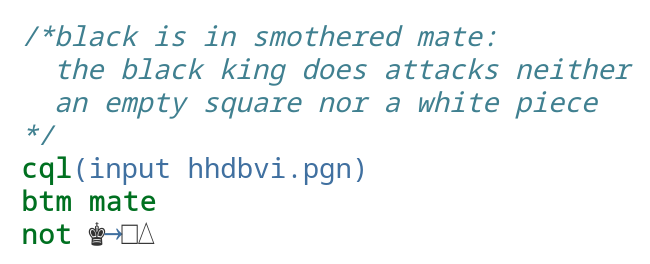
\includegraphics[width=0.45\linewidth]{background/img/cql.png}
    \caption{A CQL query to find positions where smothered mate occured.}
    \label{cql}
\end{figure}

In addition to Costeff's CQL, there exists a from-scratch clone of CQL6
\citep{cqli} which includes extra features and supports other chess variants.

This is a very powerful tool, but suffers from the same drawback as the work of
\citet{chessLanguage}: it requires extensive knowledge to use effectively. It
has been shown by \citet{cql} that CQL can support incredibly niche and complex
tactical patterns. It is possible that an expert, armed with the unsupervised
clustering (\Cref{treeS2}) and this language, can create efficient queries to
find critical chess positions.

\subsection{The Chess Transformer}\label{chessTransformerSection}

\citet{chessTransformer} demonstrate the ability of transformers to learn the
rules of chess and complex gameplay by analysing PGN games with a fine-tuned
GPT-2 transformer. By treating PGN games as a sequence of natural language
words, the authors show successful results and are able to generate new games
without specifying chess rules.

A key downside of their work is that their model generates illegal moves, which
have to be filtered manually using a chess library \citep{chessTransformer}.
This `hallucination' effect is a downside of using transformers, and other
generative techniques, in chess. 

This work is very similar to this project's work with transformers
(\Cref{mlChapter}). The key difference is that the work by
\citet{chessTransformer} operates on sequences of chess moves, while the work
in this project uses a transformer encoder to learn relationships between the
chess squares in a static position. It is unlikely that adding the extra
complexity of learning PGN outweighs the benefits, especially given the task of
this project. However, along with this project's work on transformers, the work
of \citet{chessTransformer} shows that there is potential in applying the
transformer architecture to the logical structure of chess.

\section{Future Work}\label{concS2}

\subsection{Expanding the Deep Learning Model Architecture}

A future improvement on this work is expanding the model architecture in the
transformer-based model (\Cref{mlS21}). This could involve many tricks that are
used in deep learning and transformer architectures. To supplement this, more
hyperparameter combinations could be evaluated. This would involve changing the
parts of the model that were kept constant in this work, such as learning rate,
activation functions, and number of transformer encoder layers.

This would be resource intensive, as the models take multiple hours to train,
and this could well expand to days if the model size is greatly increased.
Despite this, it is likely one of the most effective improvements on the
transformer-based model; the design and structure has been shown to be
effective, and optimising it further would be an attempt to reach its full
potential.

\subsection{Learning Latent Representations of Chess Puzzles}

Building upon the previous point, it would be interesting to experiment with a
model that attempts to learn a latent space for chess puzzles. This would
involve a contracting stage, which the current model does not have. If
successful, it could be used to group puzzles by distance within this space,
allowing very advanced clustering and similarity analysis.

Theoretically, this could be used to generate new chess positions with a
certain tactic. In practice, this would be difficult, as a small change to a
chess position changes it completely. It could also generate chess positions
that are illegal or unusual, not appearing in real games.

\subsection{Including Some Tactical Elements in Search Tree Construction}

In the current design, few tactical motifs are included when creating search
trees (\Cref{treeS13}). This was intentional, as introducing many labels could
create a biased view on what a chess puzzle truly represents. However, the work
by \citet{chessCNN} showed that including data about pinned pieces, centre
control, and vulnerable squares can improve performance. 

This will certainly improve the performance, as the current trees do not
consider moves that are impossible because of a tactic. These moves, however,
could very well be the reason why two puzzles are similar to a human player.

\subsection{Combining Both Methods}

Finally, it was mentioned that the deep learning method suffers from not having
detailed enough labels of puzzle tactics. Meanwhile, the tree-based method can
create meaningful clusters, but cannot assign any reasonable label to them
without manual checking. It may be possible to use the clustering output of the
$k$-NN algorithm and the pattern-learning transformer to extract the themes
appearing in this puzzle. 

Furthermore, by prompting the user for input, it could be possible to create an
adaptive model that can learn what a chess player thinks makes chess positions
similar. This would be an incredible leap forward and would allow automated
personalised training for chess players of all skill.

\section{Closing Remarks}\label{concS3}

This project has shown two distinct approachs to the problem of chess puzzle
analysis. Analysis of chess tactics is a topic not as often explored in chess,
as researches often focus their attention on the proving ground of
chess-playing algorithms like AlphaZero \citep{silver2018general} and Maia
Chess \citep{mcilroy2020aligning}. It is arguably more useful to the average
chess player to have greater access to higher quality chess puzzles, as
practicing these is one of the best ways of improving one's chess playing
ability.

Both methods have found success with predicting chess puzzle themes and
difficulty rating. The transformer-based model shows that this architecture has
potential for learning the structure and piece relationships in chess, while
the tree-based model shows that attempting to programmatically encode what it
means for two puzzles to be different is something that is very much feasible.

